\begin{abstract}
We demonstrate a proof of principle for using a normalizing flow to learn a physics process's probability distribution to effectively sample more data. The training data set has 5 million data points of 12 features for both $z$ and $x$ where the normalizing flow transforms $z$ to $x$. In this work, we take as input a constant 2D logistic distribution instead of $p(z)$, and examine whether the flow model can learn the transformation to $p(x)$. For simplicity, at this stage we demonstrate the method using only two features of $x$, and observed a reasonable agreement between the given physics sample and the newly-sampled data using the flow model.
\end{abstract}
\section{Introduction including Related Works }
%(we can now cite Stan's work! \textcolor{red}{did he already submit his thesis to DSpace MIT?})

Large scale particle physics experiments use humankind's largest machines to study nature at the smallest scales. One such experiment, called CLAS12 in Virginia at the Thomas Jefferson National Accelerator Facility (JLab) (\citet{BURKERT2020163419}), collides ultrarelativistic electrons moving only 1 m/s slower than the speed of light into an ultracold bunch of hydrogen to glean information about the substructure of the proton. In particular, two photons, one electron and one proton in the final state is known as Deeply Virtual $\pi^0$ Production (DV$\pi^0$P), and this process is currently under detailed study as its properties are related to the mechanical properties of the proton (\citet{PhysRevD.55.7114}).

Typically, real data is compared with the output of detailed simulations of the experiment, wherein Monte-Carlo (MC) methods are used to walk simulated particles through a detector system in many small time steps (\citet{PhysRevLett.115.212003, 10.1093/ptep/ptaa104}). The standard simulation consists of two steps. First, we generate a data set of particle features - momenta and other properties - based on a combination of field-theoretic functions and empirical physics models, which creates an `event' of a realistic four-particle final state from the DV$\pi^0$P process. This generation is very simple and computationally inexpensive. The second step is, for each event, walk all four particles through the simulated detector setup using the GEANT4 package (\citet{AGOSTINELLI2003250}). The output from this step is our four particles that we began with, but with their features smeared out. This second step is the one we are trying to supplement, as it would take about 5,000 hours on a single core machine to process 1 million events. However, through HPCC we have produced so far 100 M generated (step 1) and simulated (step 2) events that can be used for algorithmic training. 

The normalizing flow is an effective model to learn a probability distribution $p(x)$ when a sample data set $X=\{x\}$ following the distribution is given. The basic idea is a series of transformation $g_i$'s, which are referred to as flows, transforms a prior probability $p(z)$ distributions into the target distribution $p(x)$. That is
\begin{align}
    \mathbf{x} =& g_N \circ g_{N-1}\circ ... \circ g_1 (\mathbf{z}) \\
    \mathbf{z} =& f_1 \circ ... \circ f_{N-1} \circ f_N (\mathbf{x}) \label{eqn:invertible}
\end{align}
, where $f_{N-i+1}\equiv g_i^{-1}$ following \citet{9089305}'s convention. Both $\mathbf{x}$ and $\mathbf{z}$ are vectors of the same dimension $d$. From the eq.~\ref{eqn:invertible}, $g_i$ requires an invertibility condition. An intermediate flow $\mathbf{z_i}$ is defined as follows.
\begin{align}
\mathbf{z_i} =&g_i \circ ... \circ g_1(\mathbf{z}) \label{eqn:forward}\\
    =&f_{i+1}\circ ...f_N(\mathbf{x}) \label{eqn:backward}
\end{align}
, where the flow is expressed in forward direction at eq.~\ref{eqn:forward}, and in backward direction at eq.~\ref{eqn:backward}. Therefore, $\mathbf{z_{i+1}}=g_i (\mathbf{z_i})$ and $\mathbf{z_i} = f_{N-i+1}(\mathbf{z_{i+1}})$ for one flow, or layer. If the $f_i$'s are differentiable, the PDF evolves as follows.
\begin{align}
 p(\mathbf{z_{i+1}})=& p(\mathbf{z_i})|\frac{\partial f_{N-i+1}}{\partial \mathbf{z_i}}| =p(\mathbf{z_i})|\frac{\partial g_{i}^{-1}}{\partial \mathbf{z_i}}|\\
 \log p(\mathbf{z_{i+1}}) =& \log p(\mathbf{z_i}) + \log|\frac{\partial g_i^{-1}}{\partial \mathbf{z_i}}| \label{eqn:logprob}\\
 \log p(\mathbf{x}) =& \log p(\mathbf{z}) + \sum\limits_{i=1}^N \log|\frac{\partial g_i^{-1}}{\partial \mathbf{z_i}}|.
\end{align}
Eq.~\ref{eqn:logprob} is useful to define the forward and the backward propagation of each layer.
Once the NF model is trained to learn the distribution $g: p(z)\rightarrow p(x)$, it is possible to sample $x$ using sampled $z$. \citet{PhysRevD.101.076002} showed that the Nonlinear Independent Component Estimation (NICE) (\citet{Dinh15}) implementation of NF performs well by comparing the technique to existing methods in terms of efficiencies that are defined as average weight during the generation.

Motivated by \citet{stan}'s work, we use Masked Autoregressive Flows (MAF, \citet{papamakarios2018masked}), which is one of the generalized versions of NICE. The MAF starts from a simple fact that $p(z_{i}) = \prod\limits_{j}p(z_{i,j}|\mathbf{z}_{i,1:j-1})$. The component $z_{i,j}$ is the $j$-th component of $z_i$, and the vector $\mathbf{z}_{i,1:j-1}$ is defined as $\{z_{i, 1}, ..., z_{i, j-1}\}$. The transformation is finally defined as
\begin{align}
    z_{i+1, j}=& \sigma_{i, j} z_{i, j} + \mu_{i+1, j}.
\end{align}
The moments $\mu_{i+1, j}$ and $\sigma_{i, j}$ are the mean and standard deviation of $p(z_{i+1,j}|\mathbf{z}_{i+1,1:j-1})$ ($\equiv p(z_{i+1,1})$ for $j=1$). We train the flows to learn $\mu_{i+1, j}$'s and $\sigma_{i, j}$'s, and sample $p(\mathbf{x})$.

\citet{papamakarios2018masked} presents a good github repository of how to train a NF for a 2-dimensional image. The libraries are very straightforward and use PyTorch. The architecture consists of the two layers of MAF and the 2d normal prior distribution.

\section{Methods}
%We should include our work of generating the data (GEMC) and processing the data (convert to root, pandas, pickle) as these are all non-trivial steps and a good "data pipeline"
The data of 5M `events`, or sets of data points, in this problem has been achieved from Open Science Grid (OSG). The original data format is in ROOT \cite{root}, which is a widely-used format in high energy physics written in C++. There have been improvements in python libraries like uproot \cite{uproot} that can interpret the ROOT data format. The data file has been read using uproot, and saved in pickle, a standard Python library for serializing data \footnote{\url{https://github.com/6862-2021SP-team3/hipo2pickle}}. The pickled data has 5M row, each of which contains the features of four individual particles. Each individual particle has 3 features (magnitude of momentum, polar angle, azimuthal angle), so our sample $x$ has dimensions of $5\text{M}\times12$. The sampled $z$ has the same dimensions, but as sampled data points, not in the analytic distributions. \citet{Dinh15} mentions that the ``prior distribution does not need to be constant and could also be learned." We expect to learn the distribution of sample $z$'s with another NF, and use that distribution of prior in the final results. But we ignore the actual $z$ distributions, and try with the constant distributions at this stage.

\textcolor{red}{change these accordingly} We forked the repository in the organization \footnote{\url{https://github.com/6862-2021SP-team3/pytorch-normalizing-flows}}, and tested the libraries for our purpose. For the proof of the concept, we only use two columns of our data set $x$---the magnitude of electron momentum and the polar angle. We observed a good results when we used logistic distributions as prior, 12 additive alternating coupling layers, 1 output scaling layer.

\section{Preliminary Results}
The distribution in the top left subplot of Figure \ref{fig:a} shows the 2d distribution of the training data. The MAF flow was trained using a 2-dimensional logistic distribution prior, with 5,000 iterations using a sample of 1,000 training data points for each iteration. The meta-parameters of learning rate and weight decay were empirically set to 5$\times$ 10$^{-4}$ and 1$\times$10$^{-9}$, respectively. 

\begin{figure}[!ht]
    \centering
    \begin{minipage}{.5\textwidth}
        \centering
        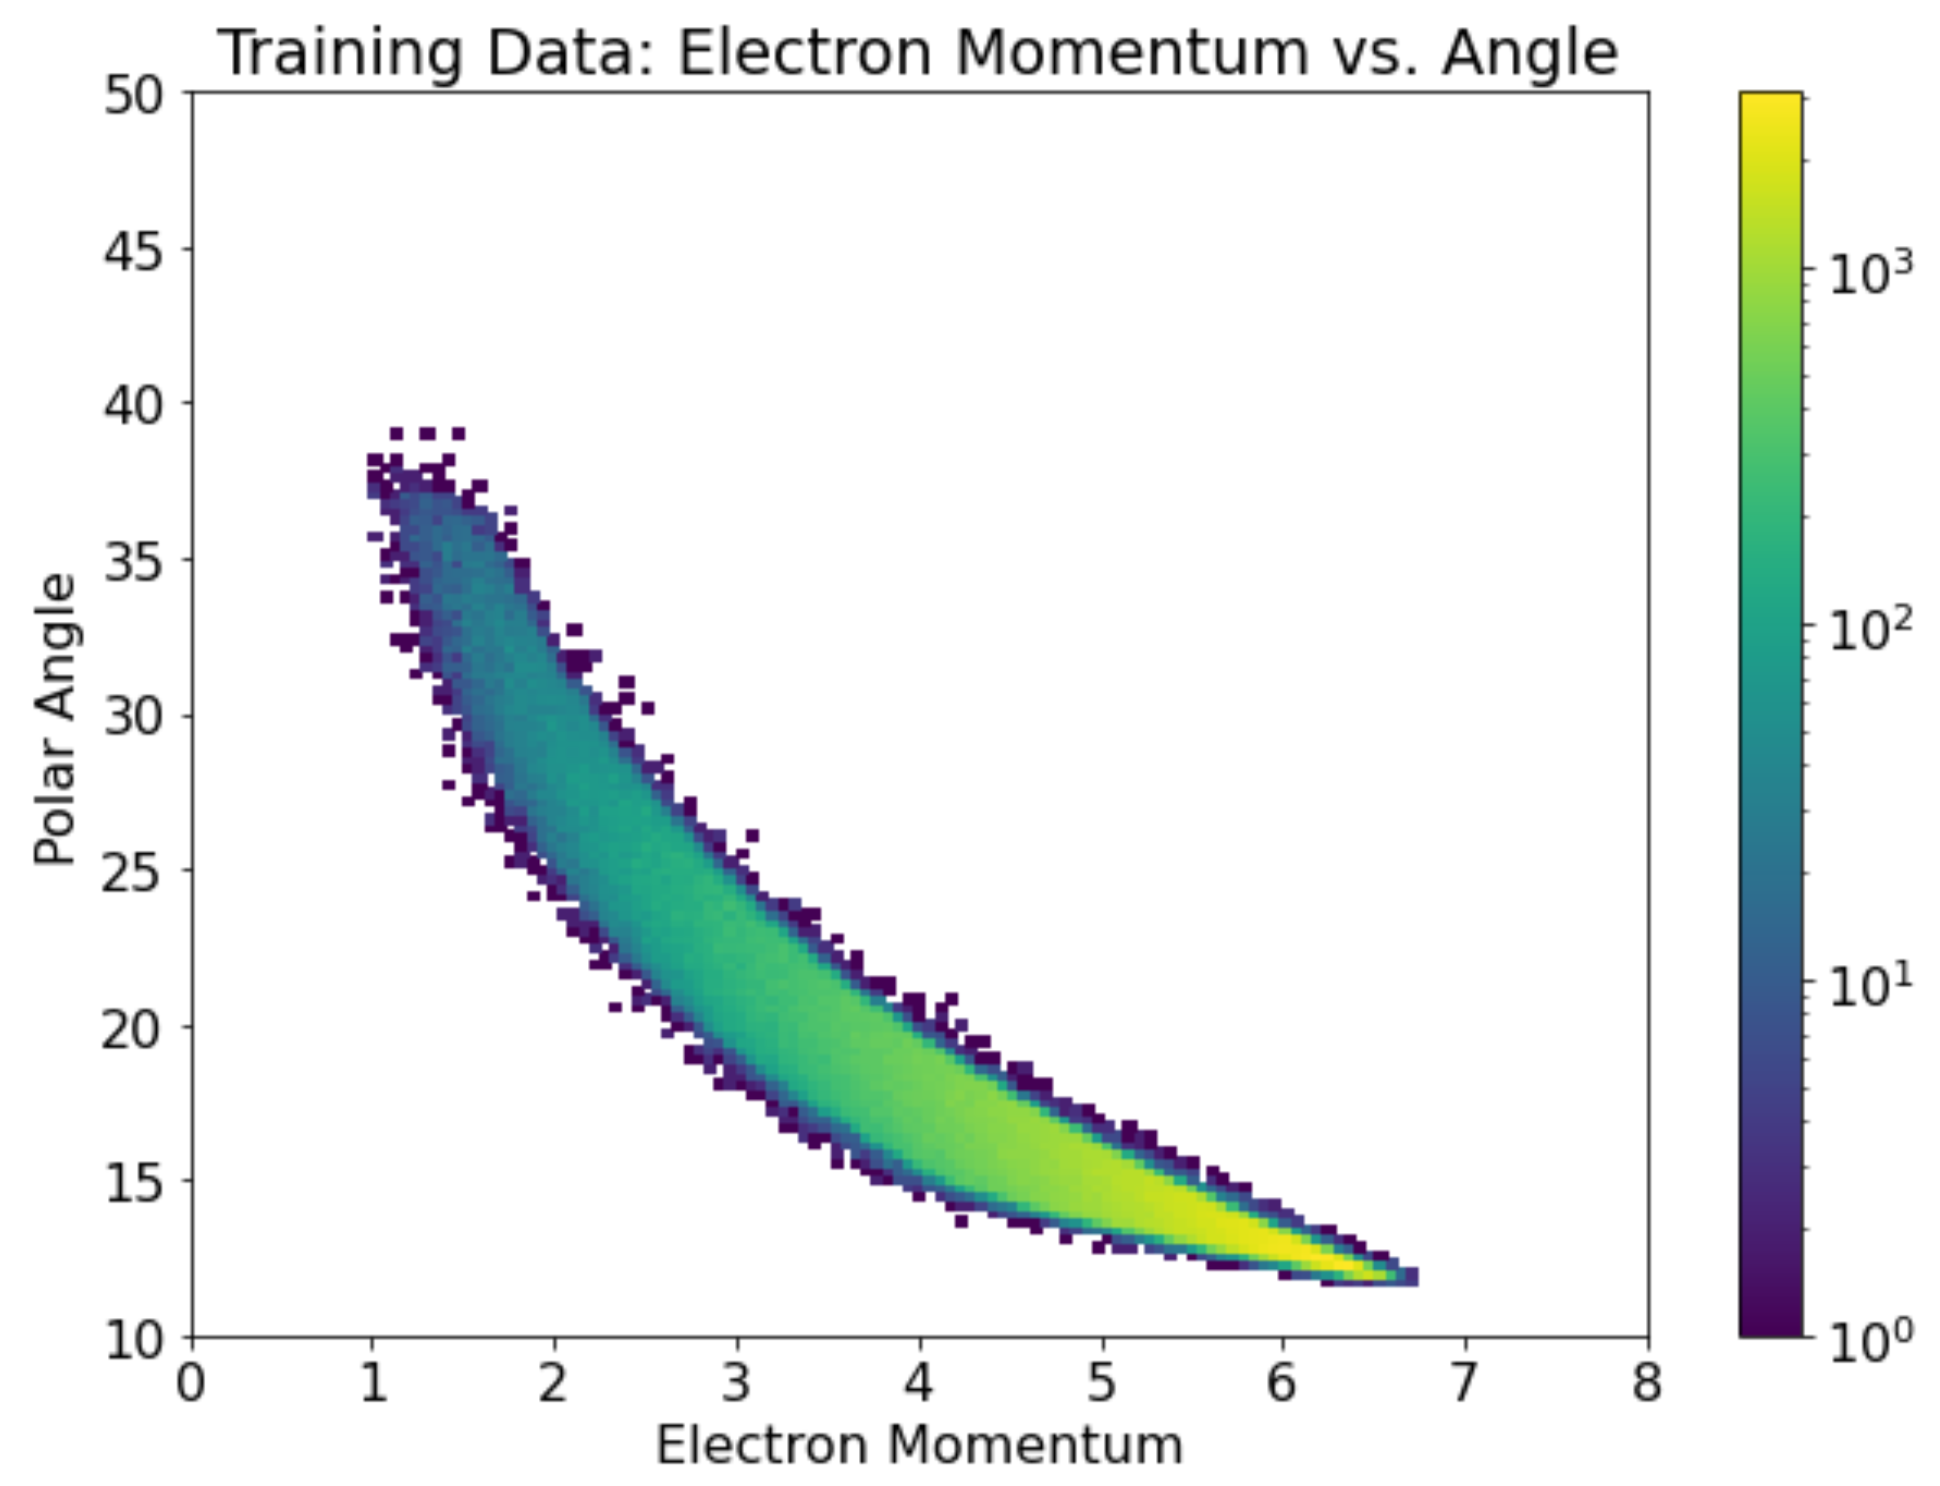
\includegraphics[width=.8\textwidth,trim={0 0 5cm 0},clip]{pictures/training_data_distribution_hires.png}
        %\caption{(a)}
        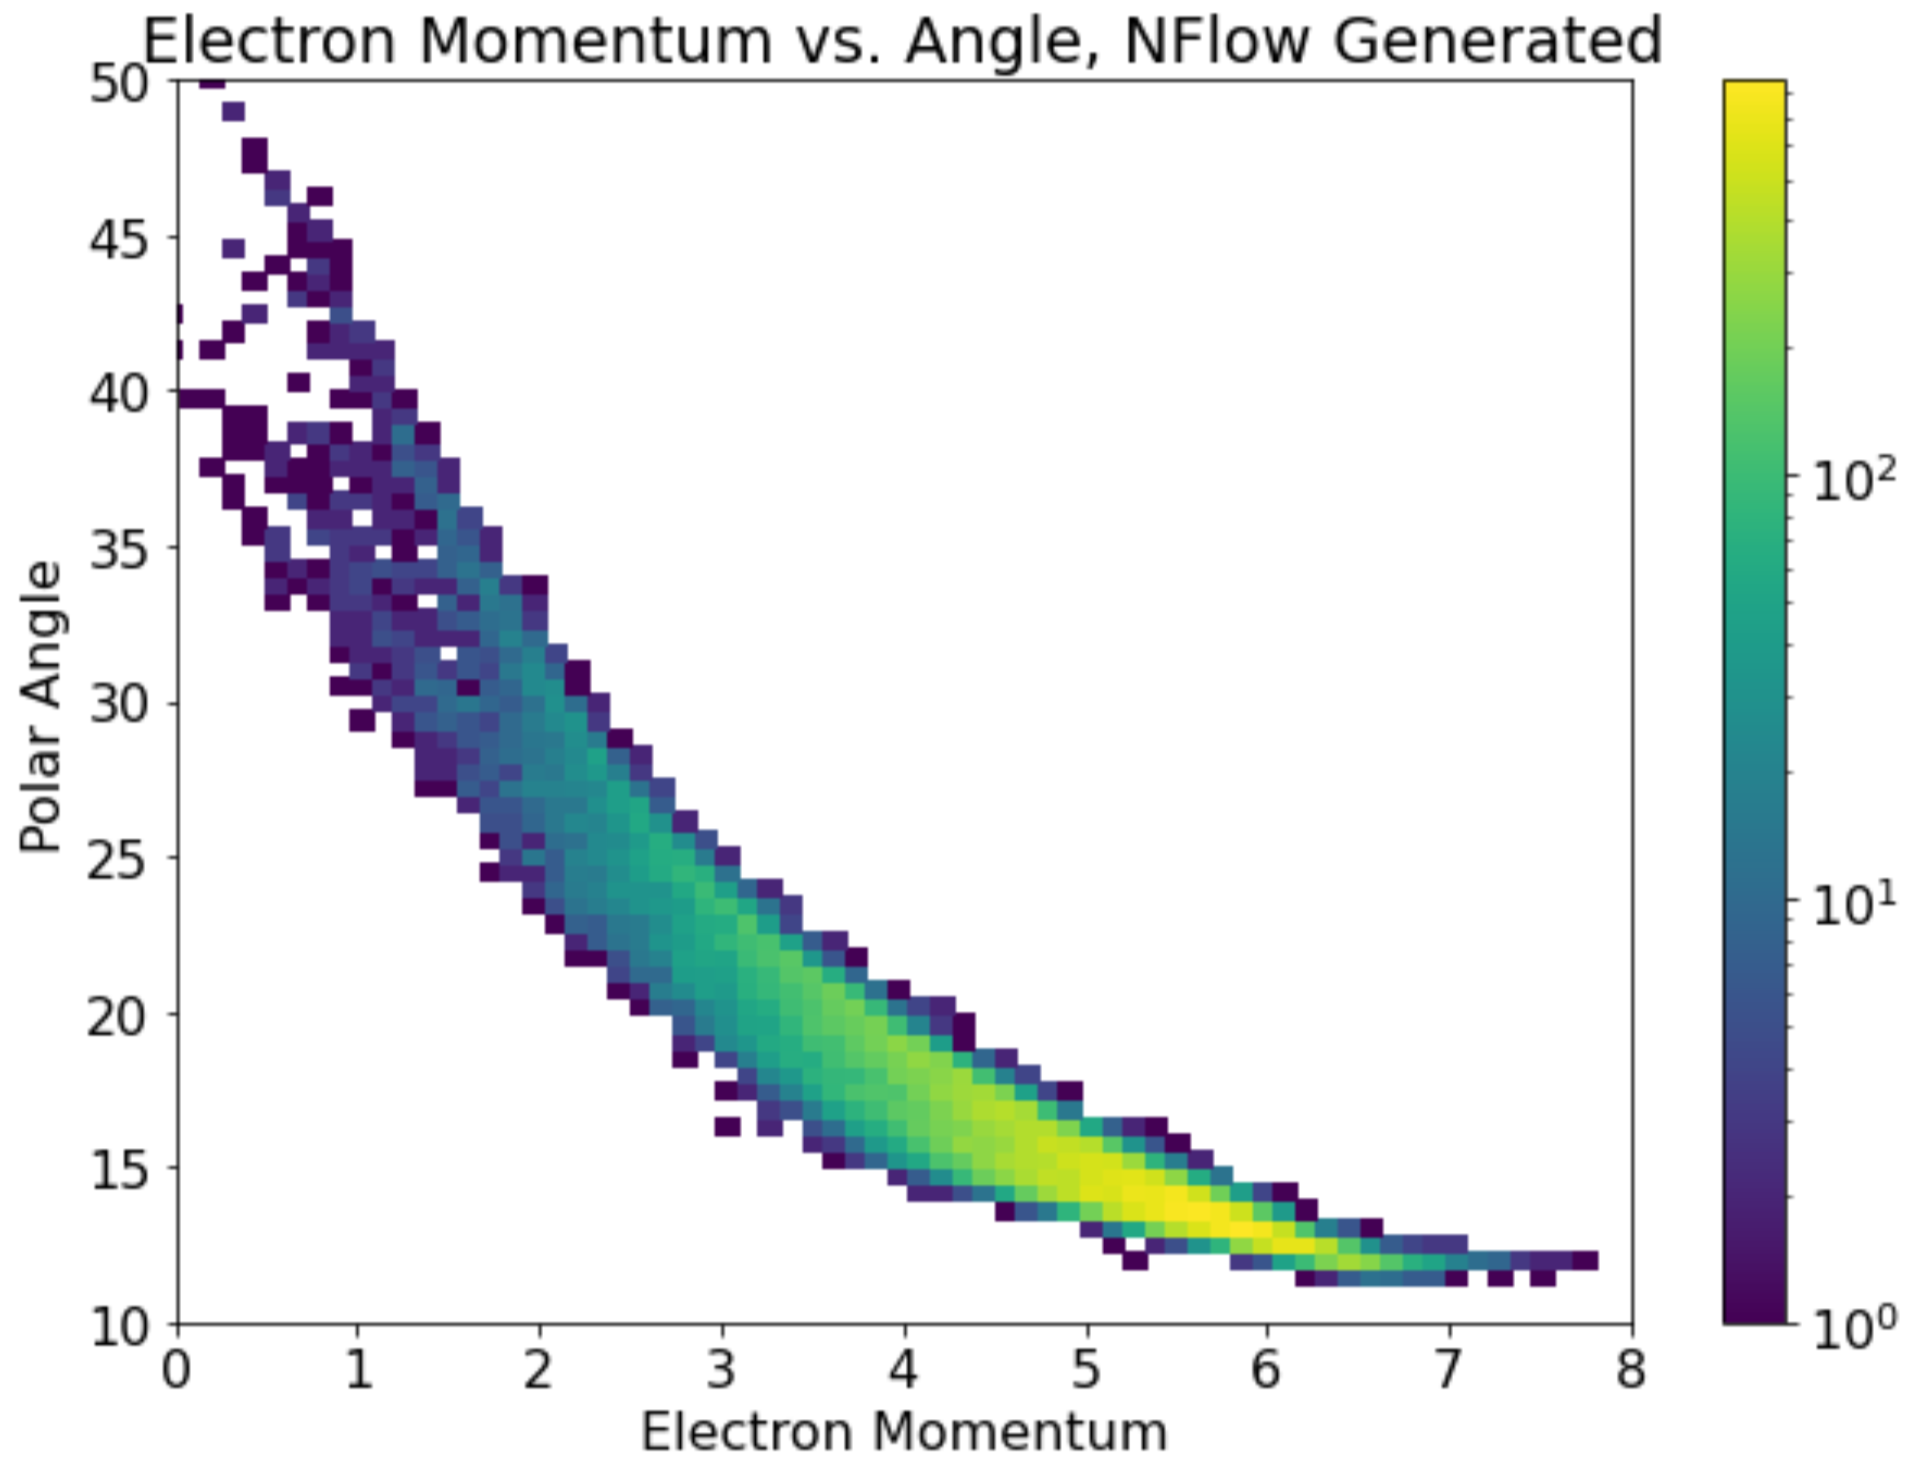
\includegraphics[width=.8\textwidth,trim={0 0 5cm 0},clip]{pictures/nflow_data_distribution_hires_0.png}
        %\caption{(c)}
    \end{minipage}%
    \begin{minipage}{0.5\textwidth}
        \centering
        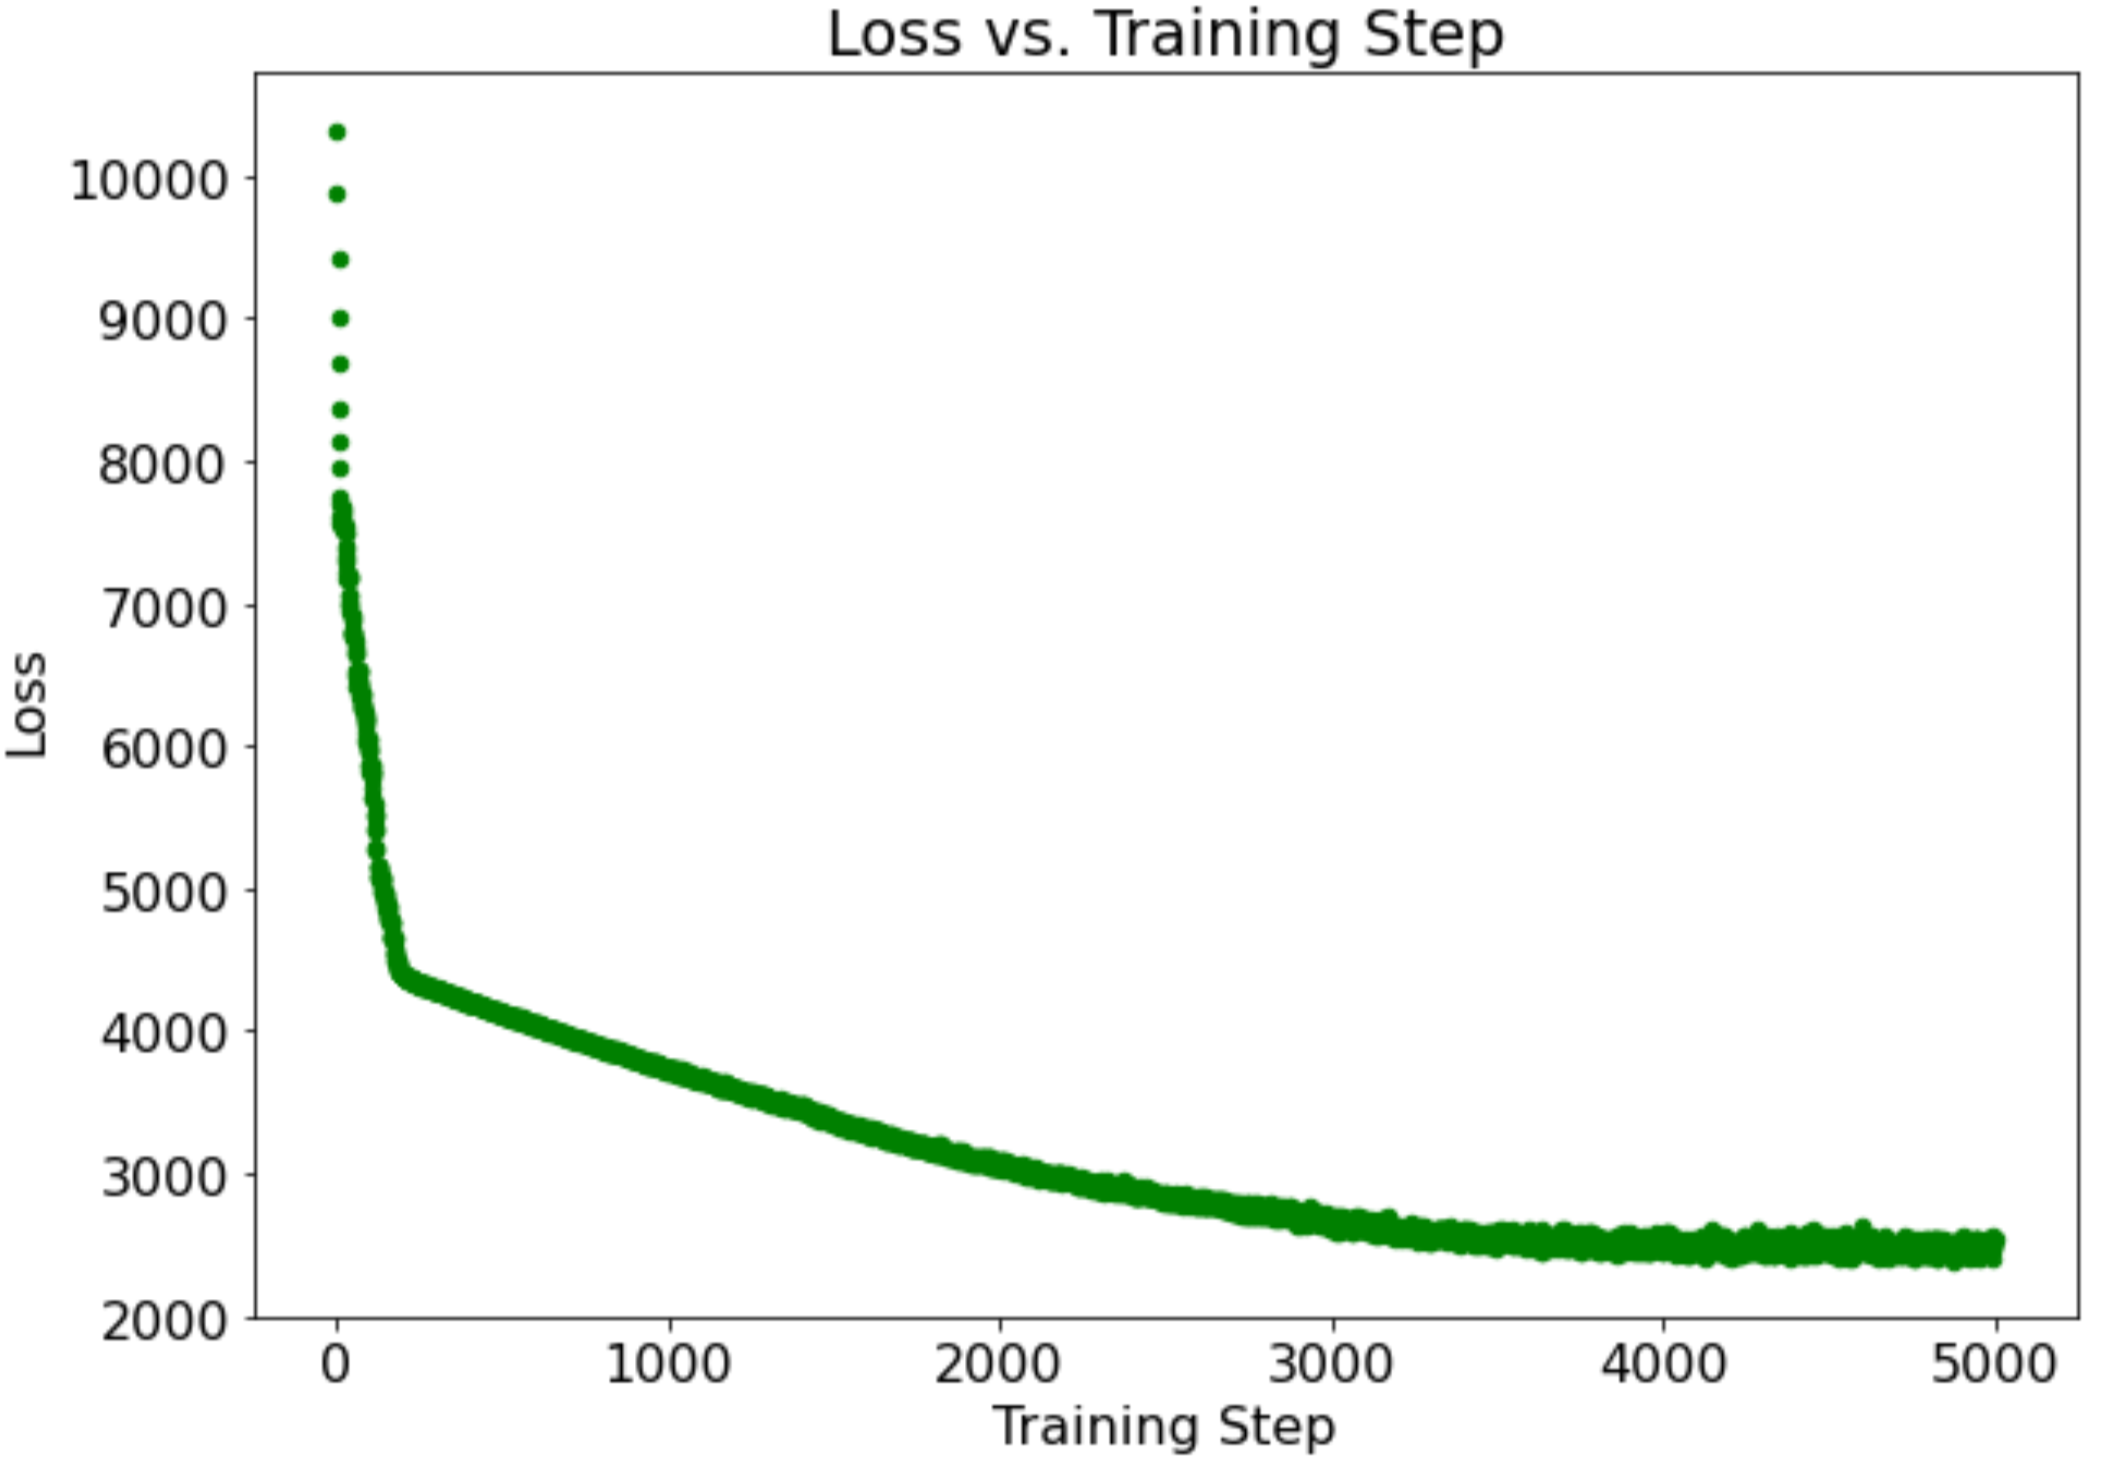
\includegraphics[width=1\textwidth,trim={0 0 0 0},clip]{pictures/loss_vs_time_2.png}
        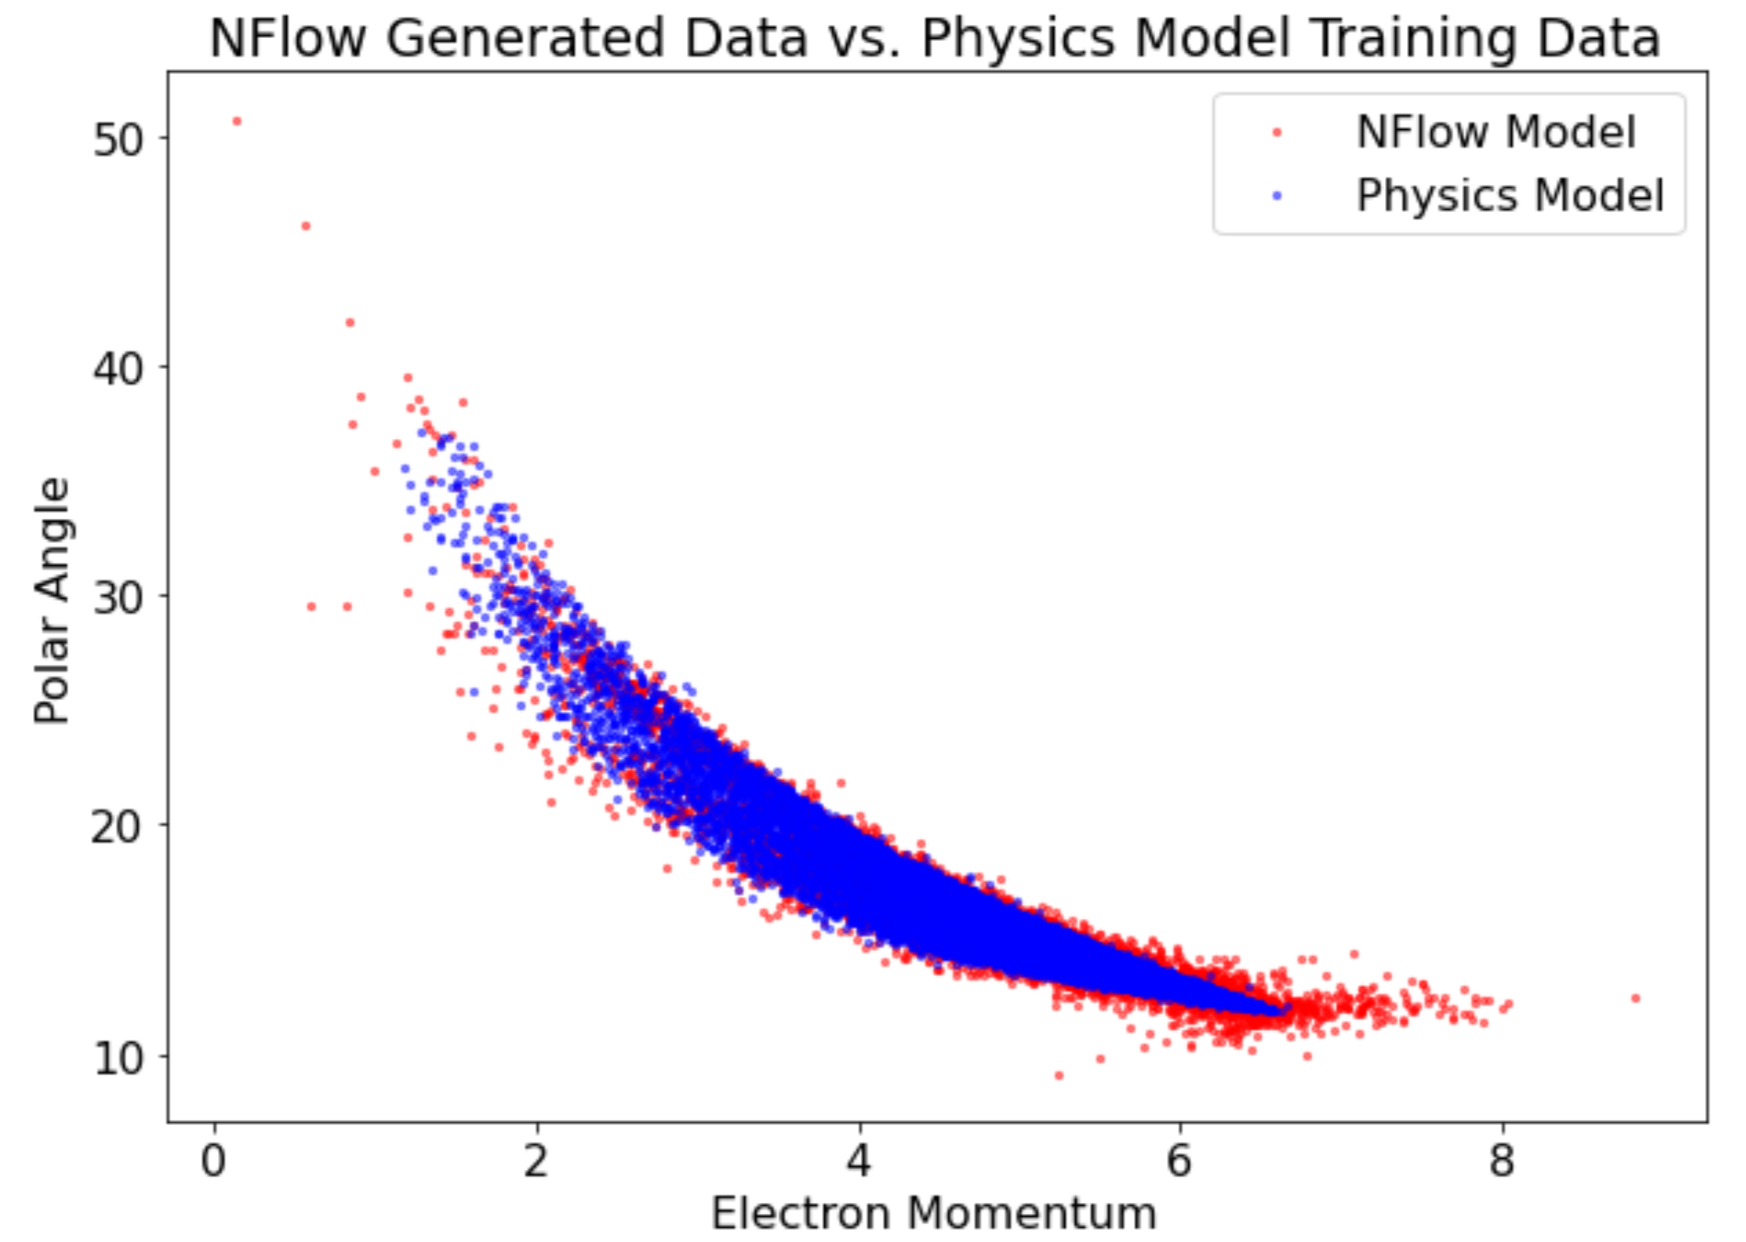
\includegraphics[width=1\textwidth,trim={0 0 0 0},clip]{pictures/nflow_vs_gemc.png}
    \end{minipage}
    \caption{Top Left: Distribution of features of training data. Top Right: Loss vs. training step. Bottom Left: Data generated from trained MAF algorithm. Bottom Right: Spatial overlay of MAF generated data and microphysics Geant4 generated data.}
    \label{fig:a}.
\end{figure}

The top right subplot of Figure \ref{fig:a} shows the training loss vs. iteration in training, from which we can see that after about 4,000 steps we converge to a minimum loss value. At this point we can use the trained model to produce data from the learned distribution, which is shown in the bottom left of Figure \ref{fig:a}.

Qualitatively, the NICE generated data is peaked around similar values, but has longer tails than the microphysics generated data. At this stage it is not clear what is causing this discrepancy, or how it can be mitigated. It is possible that including more features in training will provide higher fidelity results due to the correlations between features, but this is an active area of our research.


\section{Path Forward}


\iffalse
Path forward:\\
Utilization of "z" distribution to train prior distribution\\
Development and implementation of quantitative comparision methods\\
Expand to full feature representation learning\\
Move off of colab onto stronger computing platforms
\fi


\iffalse
Parameters for best run:

prior = TransformedDistribution(Uniform(torch.zeros(2), torch.ones(2)), SigmoidTransform().inv) # Logistic distribution
#prior = MultivariateNormal(torch.zeros(2), torch.eye(2))
# NICE
flows = [AffineHalfFlow(dim=2, parity=i%2, scale=False) for i in range(12)]
#print(flows)
flows.append(AffineConstantFlow(dim=2, shift=False))
#print(flows)


# construct the model
model = NormalizingFlowModel(prior, flows)

optimizer = optim.Adam(model.parameters(), lr=5e-4, weight\_decay=1e-9)
for k in range(5000):
    sampleDict = xz.sample(1000)
    

 Path forward:
 working just on google colab, we quickly run into computing performance issues
 \fi